
\documentclass[8pt]{beamer}

\usepackage[english]{babel}
\usepackage[utf8]{inputenc}
\usepackage{pdfpages}
\usepackage{color}
\usepackage{graphicx, import}
\usepackage{amsmath}
\usepackage{amssymb}
\usepackage{physics} % norm
\usepackage{tikz}
\usepackage{tkz-euclide}
\usepackage{pgfplots}
\usepackage{tabularx}
\usepackage[numbers, square]{natbib}
\usepackage{mathtools}
\usepackage{transparent}
\usepackage{caption} % change style of figure 
\usepackage{subcaption}
\usepackage{booktabs}
\usepackage[super]{nth}

\captionsetup*[subfigure]{position=bottom}


\usetikzlibrary{positioning, fit, patterns, snakes, chains, arrows, decorations.markings, arrows.meta}
%\tikzexternalize[prefix=out/figures/]
\newcolumntype{Y}{>{\centering\arraybackslash}X} % centered equidistant columns

\bibliographystyle{plainnat}
\usetheme{metropolis}
\setbeamertemplate{frame footer}{\insertshortauthor\hfill\insertshortinstitute}
\setbeamercolor{footline}{fg=gray}

\DeclareMathOperator{\loss}{loss}


\title[]{Effects of Pose Normalization on\\ Weakly Supervised 3D Human Pose Estimation}
\author[Nikolas Klug]{Nikolas Klug}
\institute[University of Augsburg]{University of Augsburg}
\date{\nth{6} November 2019}


\begin{document}
	{
	\setbeamertemplate{footline}{}
	\begin{frame}
		\titlepage
	\end{frame}
	}
	\addtocounter{framenumber}{-1}

	\begin{frame}{Source}
		\textbf{Can 3D Pose be Learned from 2D Projections Alone?}\linebreak
		\begin{footnotesize}
			Dylan Drover, Rohith MV, Ching-Hang Chen, Amit Agrawal, Ambrish Tyagi, and Cong Phuoc Huynh.\linebreak
			In Computer Vision -- ECCV 2018 Workshops, Pages 78-94, 2019. Springer International Publishing.
		\end{footnotesize}
	\end{frame}

%	\begin{frame}{Why?}
%		\begin{itemize}
%			\item Very good 2D keypoint detectors out there: Stacked Hourglass, OpenPose etc.
%			\item Massive amount of 2D images/videos available
%			\item Acquiring 3D ground truth data is cumbersome and expensive
%		\end{itemize}
%	\end{frame}

	\begin{frame}{How It Works}
		\begin{figure}
			\centering
			\makebox[\textwidth][c]{
				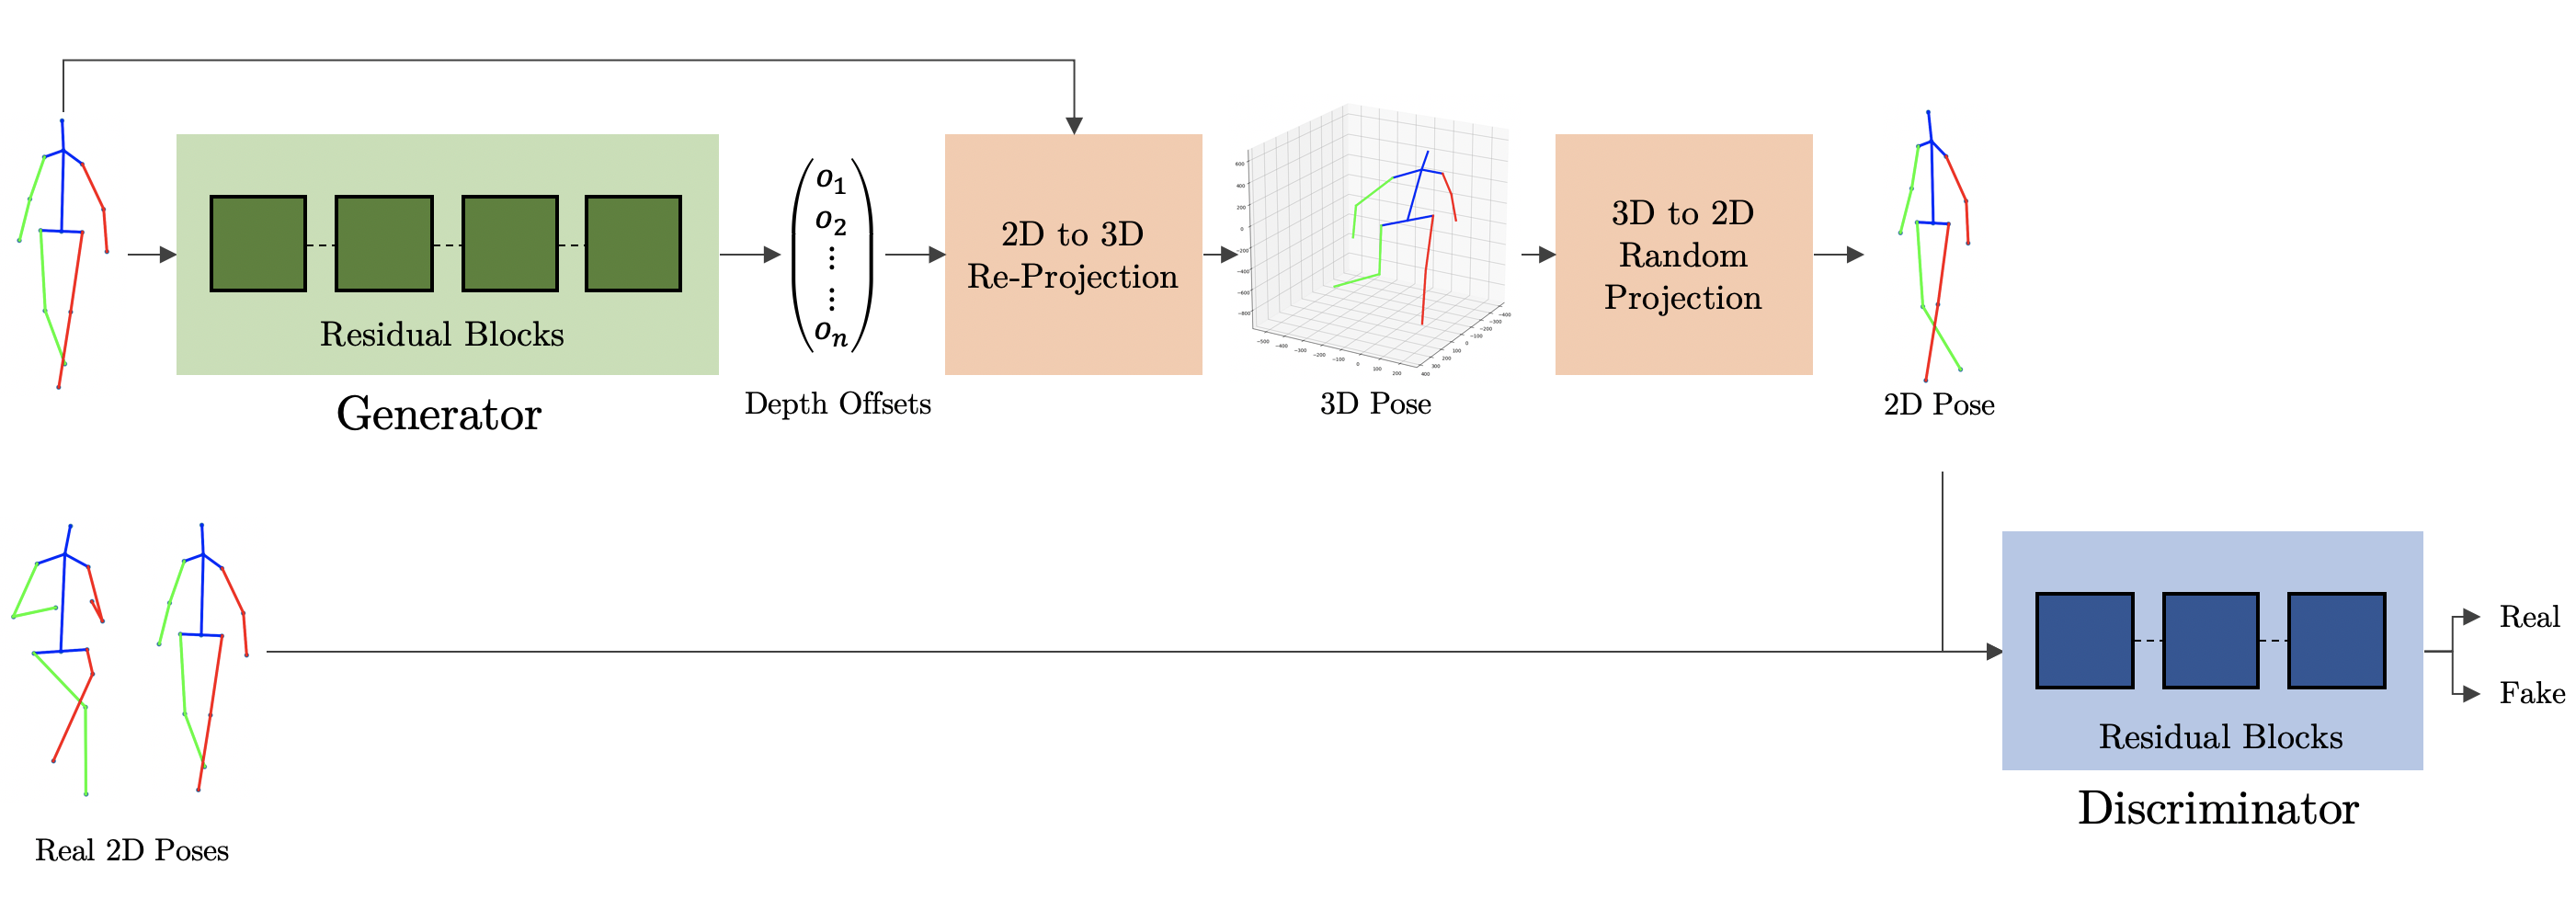
\includegraphics[width=1.1\textwidth]{figures/system.png}
			}                
		\end{figure}
	\end{frame}

	\begin{frame}{Baseline Results}
		\begin{table}
			\centering
			\begin{tabularx}{\textwidth}{l *{8}{Y}}
				\toprule
				Method & Direct. & Discuss & Eat & Greet & Phone & Pose & Purchase & Sit \\
				\midrule
				\citet{drover18} & 34.3 & 36.4 & 28.4 & 33.7 & 30.0 & 43.8 & 31.7 & 32.5\\
				Protocol 1 & 36.3 & 35.5 & 35.6 & 42.6 & 34.8 & 44.1 & 45.2 & 36.3 \\
				Protocol 2 & 48.8 & 51.5 & 41.5 & 57.7 & 49.4 & 54.3 & 48.8 & 50.0 \\
				\bottomrule
				\toprule
				Method & SitDown & Smoke & TPhoto & Wait & Walk & WDog & WTog. & \textbf{Avg.}\\
				\midrule
				\citet{drover18} & 48.9 & 32.1 & 43.8 & 36.0 & 25.1 & 34.1 & 30.3 & \textbf{34.2}\\
				Protocol 1  & 51.9 & 41.9 & 50.8 & 43.0 & 38.5 & 49.6 & 40.8 & \textbf{41.0} \\
				Protocol 2 & 64.3 & 51.9 & 64.6 & 57.1 & 54.3 & 57.9 & 53.2 & \textbf{54.8} \\
				\bottomrule
			\end{tabularx}
		\caption{Mean Per Joint Position Errors reported in \cite{drover18} (Protocol 1) and for synthetic poses from the Human3.6M dataset for Protocol 1 (w/ rotation)  and Protocol 2 (w/o rotation). 
			The MPJPEs are given in millimeters.}
		\end{table}
	\end{frame}

	
	\begin{frame}[t]{Constraints and Normalization}
		Constraints:
		\begin{itemize}
			\item[(A)] The 2D input pose's root joint is centered at the origin of the image plane.
			\item[(B)] A designated norm limb has length 0.1.
		\end{itemize}
		\vfill
		\begin{figure}
			\hspace{-.5cm}
			\centering{
			\uncover<2->{
			\begin{subfigure}{.45\textwidth}
			\begin{tikzpicture}
				\draw[->] (0,0) -- (1.5,0);
				\draw[->] (0,0) -- (0,1.5);
				\tkzDefPoint(1.5,0){x}
				\tkzDefPoint(0,1.5){y}
				\tkzLabelPoint[left](y){\tiny{y}}
				\tkzLabelPoint[above](x){\tiny{x}}
				\node[] (origin) at (0,0) [circle, fill, inner sep=1.5pt]{};
				\node[] (shifted) at (-2,1) [yshift=-2pt, xshift=-1pt]
				{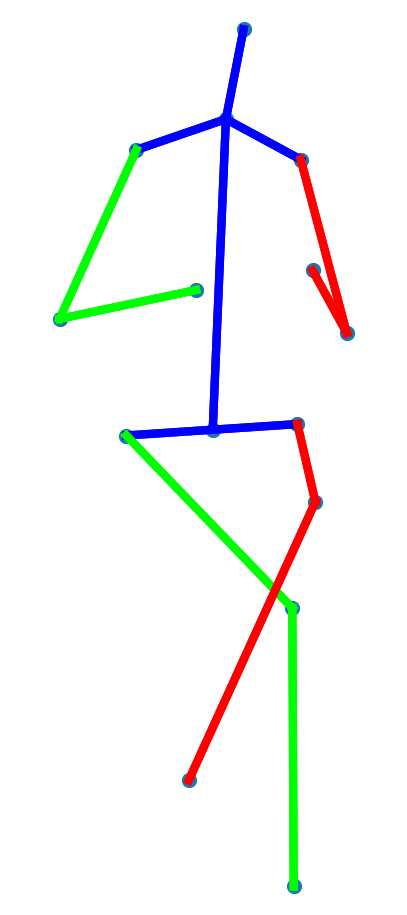
\includegraphics[width=.2\textwidth]{figures/2D_pose_514651_transparent.png}};
				\node[] (normalized) at (0,0) [yshift=-2pt, xshift=-1pt]
				{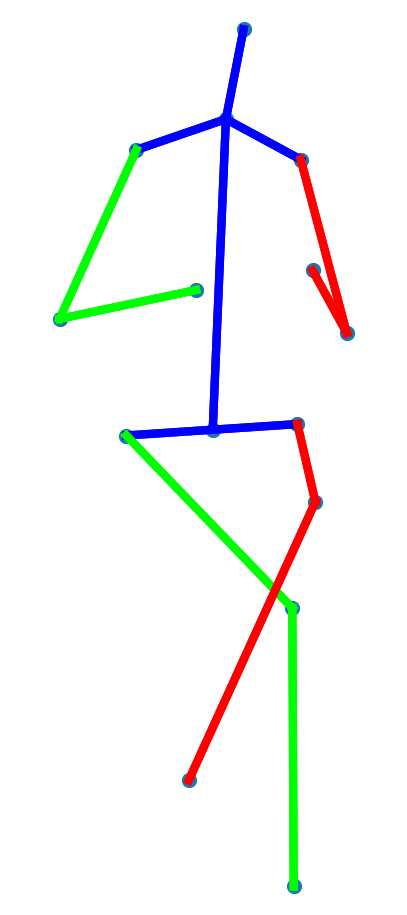
\includegraphics[width=.2\textwidth]{figures/2D_pose_514651_transparent.png}};
				\draw[-Latex, line width=1pt, dashed, shorten >=0.2cm, shorten <=.2cm] (-2, 1) -- (0,0);
				\tkzLabelPoint[below left= .06cm of origin](origin){\tiny{$(0,0)$}};
			\end{tikzpicture}
			\vspace{1.4mm}
			\subcaption{Normalization by translation}
			\end{subfigure}
			}\hfill
			\begin{subfigure}{.45\textwidth}
				\uncover<3->{\begin{tikzpicture}
					\draw[->] (0,0) -- (1.5,0);
					\draw[->] (0,0) -- (0,1.5);
					\tkzDefPoint(1.5,0){x}
					\tkzDefPoint(0,1.5){y}
					\tkzLabelPoint[left](y){\tiny{y}}
					\tkzLabelPoint[above](x){\tiny{x}}
					\node[] (scaled) at (0,0) [yshift=-2pt, xshift=-1pt]
					{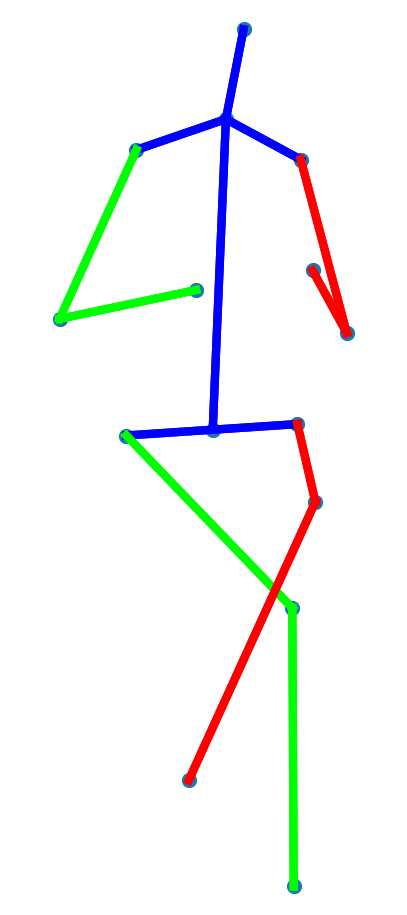
\includegraphics[width=.3\textwidth]{figures/2D_pose_514651_transparent.png}};
					\node[] (origin) at (0,0) [circle, fill, inner sep=1.5pt]{};
%					\draw[to-to, line width=0.5pt, dashed](-0.7, 1.5) -- (-0.7, -1.64);
					\tkzLabelPoint[below left= .6mm of origin](origin){\tiny{$(0,0)$}};
					\draw[->] (3.5,0) -- (5,0);
					\draw[->] (3.5,0) -- (3.5,1.5);
					\tkzDefPoint(5,0){x1}
					\tkzDefPoint(3.5,1.5){y1}
					\tkzLabelPoint[left](y1){\tiny{y}}
					\tkzLabelPoint[above](x1){\tiny{x}}
					\node[] (normalized) at (3.5,0) [yshift=-2pt, xshift=-1pt]
					{{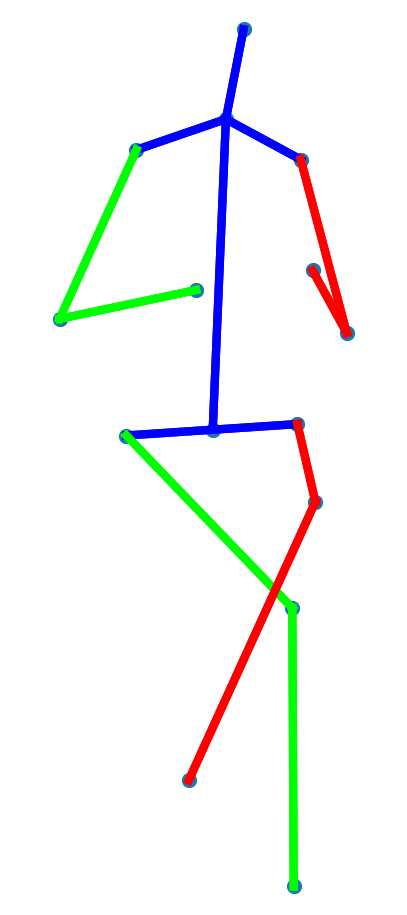
\includegraphics[width=.2\textwidth]{figures/2D_pose_514651_transparent.png}}};
					\node[] (origin1) at (3.5,0) [circle, fill, inner sep=1.5pt]{};
					\tkzLabelPoint[below left= .6mm and -1mm of origin](origin1){\tiny{$(0,0)$}};
%					\draw[line width=0.5pt, dashed, to-to] (3, 0.98) -- (3, -1.12);
					\draw[-Latex, line width=1pt, dashed] (1.5, 0.3) -- (2.5, 0.3);
				\end{tikzpicture}
			\subcaption{Normalization by scaling}
			}
			\end{subfigure}
		}
		\hspace{.5cm}
		\end{figure}
		\vfill

	\end{frame}

	\begin{frame}{Effects of Pose Normalization by Translation}
	Theoretical lower bound for the MPJPE caused by translation:
	\begin{equation*}
		\Delta d(X_i, Y_i, Z_i, dx, Z) = \abs{dx \left (\frac{1}{Z_i} - \frac{1}{Z} \right )} \sqrt{\frac{Y_i^2 + Z_i^2}{1 + a^2 + b^2}} \ , 
	\end{equation*}
	where:
	\begin{itemize}
		\item $dx$: offset along the x axis
		\item $(X_i, Y_i, Z_i)$: joint of the pose $P$
		\item $Z$: absolute distance between the camera and $P$'s root joint
		\item $a = \left( \frac{X_i}{Z_i} + dx \left( \frac{1}{Z_i} - \frac{1}{Z} \right) \right )$
		\item $b = \frac{Y_i}{Z_i}$
	\end{itemize}  
	\end{frame}

	\begin{frame}{Experimental and theoretical MPJPEs caused by translation}
		\begin{figure}
	\begin{subfigure}[]{.45\textwidth}
		\centering
		\begin{tikzpicture}[trim axis left]
			\begin{axis}[
			tiny,
			width=1.25\textwidth,
			xlabel={$dx$ [m]},
			%			axis lines = middle,
			y label style={at={(axis description cs:0.1,1.1)},rotate=-90,anchor=north},
			ylabel={MPJPE [mm]},
			grid=both,
			enlarge x limits = false,
			grid style={draw=gray!50},
			minor tick num = 1,
			tick style={draw=gray!50},
			xtick={-100,-50,0,50,100},
			extra x ticks={0},
			scaled x ticks = false,
			no markers,
			every axis plot/.append style={}
			]
			\addplot table [x=a, y=b, col sep=comma] {figures/plot_e_03_07_original_x_shift.csv};
			\addplot table [x=a, y=b, col sep=comma] {figures/plot_theoretical_x_shift_scaled.csv};
			\end{axis}
			\end{tikzpicture}
	\end{subfigure}\hfill
	\begin{subfigure}[]{.45\textwidth}
		\centering
		\begin{tikzpicture}[trim axis left]
		\begin{axis}[
		tiny,
		width=1.25\textwidth,
		xlabel={$dx$ [m]},
		%			axis lines = middle,
		y label style={at={(axis description cs:0.1,1.1)},rotate=-90,anchor=north},
		ylabel={MPJPE [mm]},
		grid=both,
		enlarge x limits = false,
		grid style={draw=gray!50},
		minor tick num = 1,
		tick style={draw=gray!50},
		xtick={-3,-2,-1,0,1,2,3},
		extra x ticks={0},
		scaled x ticks = false,
		no markers,
		every axis plot/.append style={}
		]
		\addplot +[restrict expr to domain={\coordindex}{180:401}] table [x=a, y=b, col sep=comma] {figures/plot_e_03_07_original_x_shift.csv};
		\addplot +[restrict expr to domain={\coordindex}{180:401}] table [x=a, y=b, col sep=comma] {figures/plot_theoretical_x_shift_scaled.csv};
		\end{axis}
		\end{tikzpicture}
	\end{subfigure}
	\caption{Theoretical (red) and experimental (blue) MPJPEs for different values of $dx$ without rotation.
		The distance between the camera and the poses is ten times the norm limb length (approximately 5m).}
\end{figure}
	\end{frame}

	\begin{frame}{Experimental and theoretical MPJPEs caused by scaling}
		\begin{figure}
		\centering
		\begin{tikzpicture}[trim axis left]
		\begin{axis}[
		tiny,
		width=\textwidth,
		height=6cm,
		xlabel={$dz$ [m]},
		%			axis lines = middle,
		y label style={at={(axis description cs:0.12,1.08)},rotate=-90,anchor=north},
		ylabel={MPJPE [mm]},
		grid=both,
		enlarge x limits = false,
		grid style={draw=gray!50},
		minor tick num = 1,
		tick style={draw=gray!50},
		scaled x ticks = false,
		no markers,
		xtick={-3,-2,...,15},
		every axis plot/.append style={}
		]
		\addplot table [x=a, y=b, col sep=comma] {figures/plot_e_03_07_original_z_shift.csv};
		\addplot table [x=a, y=b, col sep=comma] {figures/plot_theoretical_z_shift_scaled.csv};
		\end{axis}
		\end{tikzpicture}
	\caption{Experimental (blue) and theoretical (red) MPJPEs for different values of $dz$.
		The distance between the camera and the poses is ten times the norm limb length (approximately 5m).
	}
	\label{fig:z-shift-error}
\end{figure}
	\end{frame}

	\begin{frame}{Network modification}
		Prevention of the increased MPJPE (caused by translation):
		\begin{itemize}
			\item 2D poses are shifted back before re-projection into 3D
			\item Removal of the normalization constraint and training with non-normalized poses
		\end{itemize}
		\begin{figure}
			\centering
			\makebox[\textwidth][c]{
				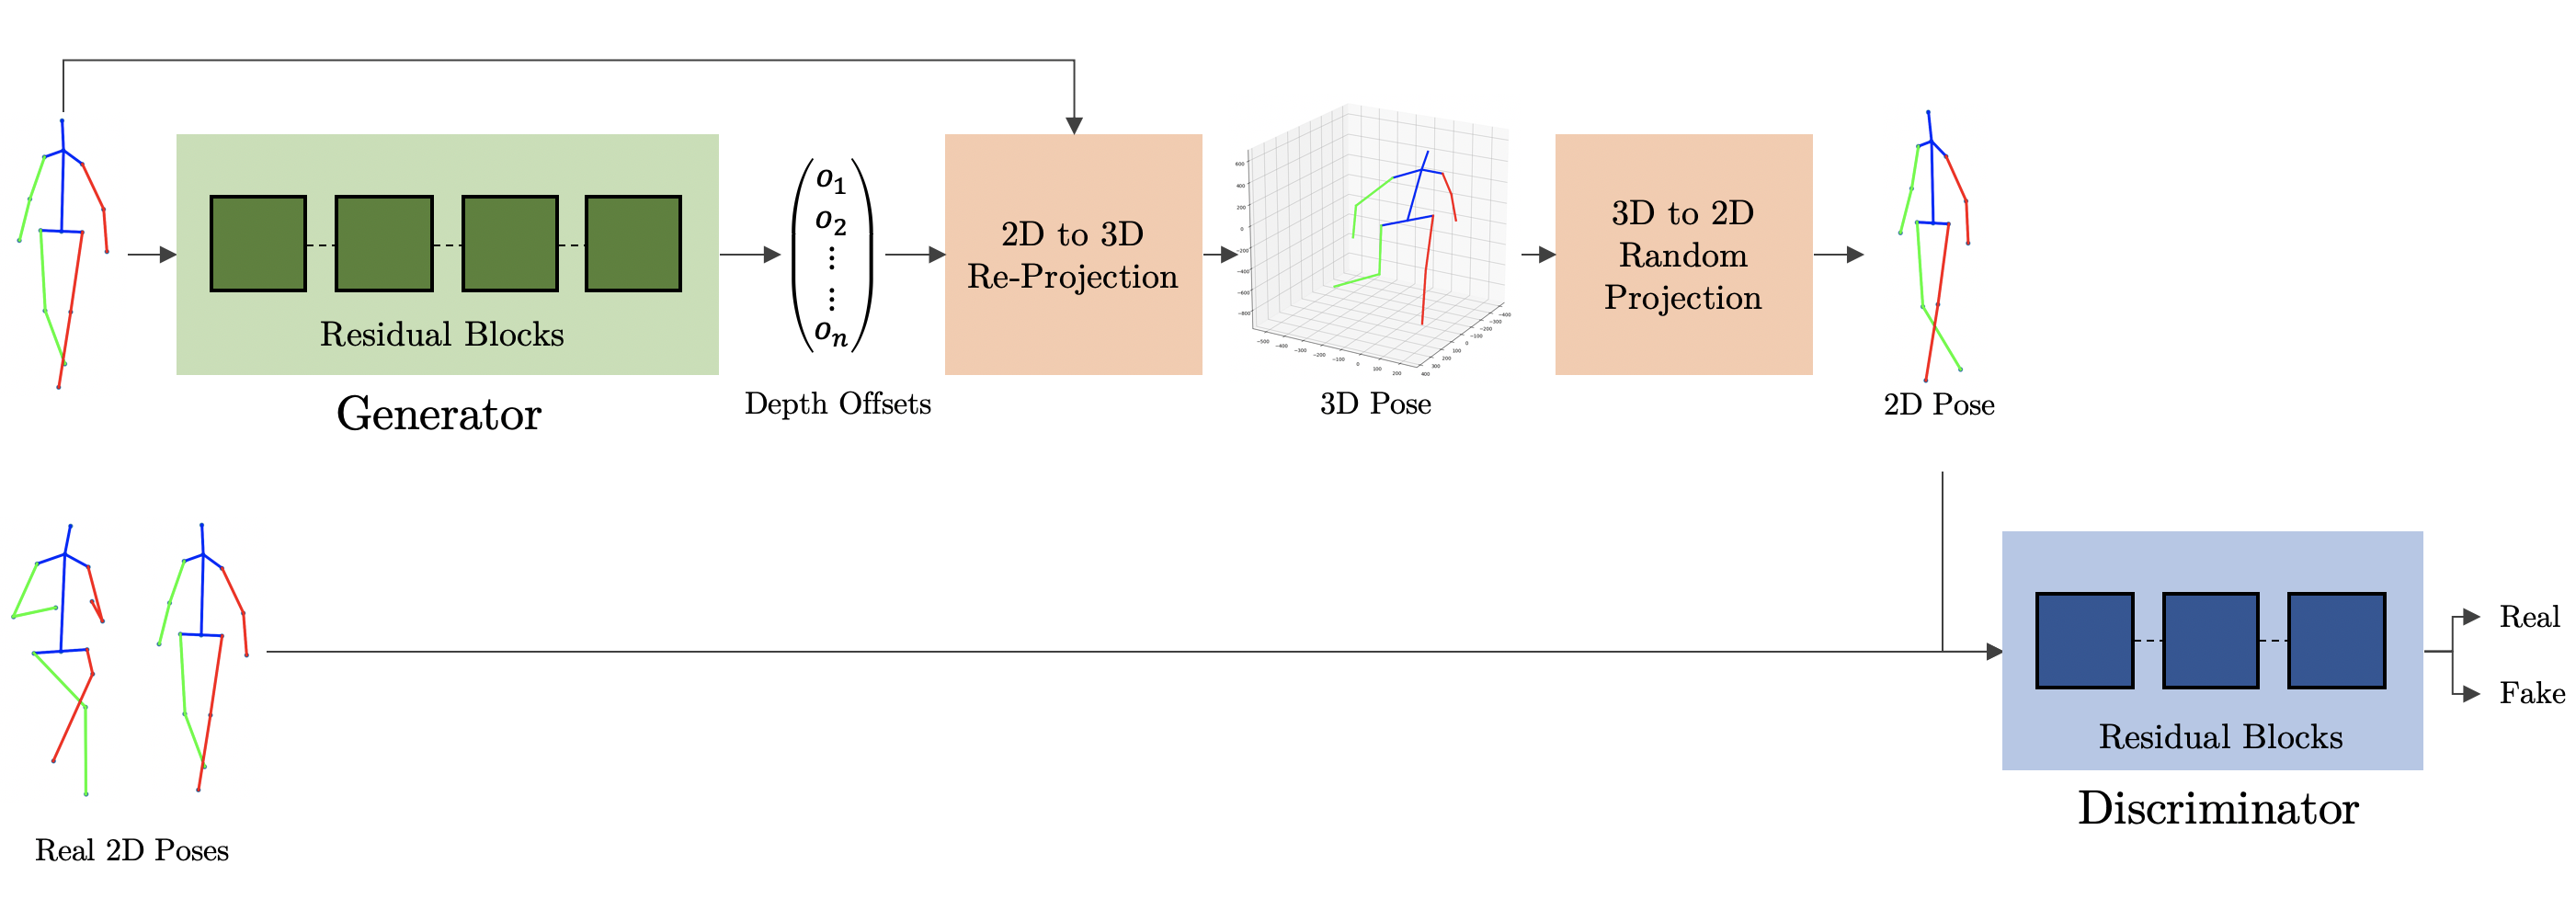
\includegraphics[width=1.1\textwidth]{figures/system.png}
			}                
		\end{figure}
	\end{frame}

	\begin{frame}{Results for Modified Network}
		\begin{figure}
			\begin{subfigure}[]{.63\textwidth}
				\centering
				\begin{tikzpicture}[trim axis left]
				\begin{axis}[
				tiny,
				width=1.25\textwidth,
				xlabel={$dx$ [m]},
				%			axis lines = middle,
				y label style={at={(axis description cs:0.05,1.07)},rotate=-90,anchor=north},
				ylabel={MPJPE [mm]},
				grid=both,
				enlarge x limits = false,
				grid style={draw=gray!50},
				minor tick num = 1,
				tick style={draw=gray!50},
%				xtick={-3,-2,-1,0,1,2,3},
				extra x ticks={0},
				scaled x ticks = false,
				no markers,
				every axis plot/.append style={}
				]
				\addplot +[restrict expr to domain={\coordindex}{90:491}] table [x=a, y=b, col sep=comma] {figures/plot_e_03_07_original_x_shift.csv};
				\addplot[color=black!60!green] table [x=a, y=b, col sep=comma] {figures/plot_e_01_06_shifted_generator_x_shift.csv};
				\end{axis}
				\end{tikzpicture}
			\end{subfigure}
			\caption{MPJPEs for original (blue) and modified (green) network for different values of $dx$ without rotation.
				The distance between the camera and the poses is approximately 5m.}
\end{figure}
	\end{frame}

	\begin{frame}[t]{Introduction of Limb Loss}
		\vfill
		Limb $l = (u, v)$: Connecting body part between vertices $u$ and $v$.\\
		Set of symmetric limbs $S \coloneqq \{(l_{i_1}, l_{i_2})~|~ l_{i_1}, l_{i_2}\ \text{are symmetric limbs} \}$\\
		\vfill
		\textbf{Limb Loss}:
		Punishes the generator if it produces 3D poses with symmetric limbs of different lengths
		\vspace{2em}
		\begin{align*}
		&\loss_{limb} \coloneqq \frac{1}{|S|}\sum_{((u_1, v_1), (u_2, v_2)) \in S} \bigl\lvert \norm{u_1 - v_1}_2 - \norm{u_2 - v_2}_2 \bigr\rvert\\[1em]
		&\loss_{G, limb} \coloneqq \loss_G + \lambda \cdot \loss_{limb}
		\end{align*}	
		\vfill	
	\end{frame}
	
	\begin{frame}{Results for Limb Loss}
		\begin{table}[bt]	
		\centering
		\begin{tabularx}{\textwidth}{l *{8}{Y}}
			\toprule
			Method & Direct. & Discuss & Eat & Greet & Phone & Pose & Purchase & Sit \\
			\midrule
			$loss_G$ & 48.2 & 52.9 & 47.4 & 58.7 & 54.3 & 57.6 & 51.7 & 52.5\\
			$loss_{G, limb}$ & 42.9 & 51.6 & 41.9 & 55.0 & 49.2 & 51.6 & 51.1 & 45.9 \\
			\bottomrule
			\toprule
			Method & SitDown & Smoke & TPhoto & Wait & Walk & WDog & WTog. & \textbf{Avg.}\\
			\midrule
			$loss_G$ & 64.3 & 51.9 & 64.6 & 57.1 & 54.3 & 57.9 & 53.2 & \textbf{54.8} \\
			$loss_{G, limb}$ & 61.0 & 47.0 & 61.4 & 54.4 & 45.7 & 56.7 & 48.1 & \textbf{50.7} \\
			\bottomrule
		\end{tabularx}
		\caption{
			Comparison of the MPJPEs with standard and modified loss for the Human3.6M dataset without rotation. The MPJPEs are given in millimeters.
		}
		\label{tbl:results-limb-loss}
		\end{table}
	\end{frame}


	\begin{frame}
		\bibliography{bibliography}
		\bibliographystyle{plainnat}
	\end{frame}
\end{document}